\section{Experiments} %TODO: Subsections
\label{results}
%From ILO:
%"Plan and carry out a small-scale investigation of an algorithmic research problem. This investigation could be theoretical, experimental, or both."
This section describes the results reached in the project. The goal in this section is threefold. (1) to verify the results achieved in \cite{wagner17}. (2) to explore the performance of \qs{} on new datasets. (3) to discover the performance of \qsr{} and compare this to the performance of \qs{}.
\\
\\
%The expirements are based on two datasets from the paper(\sift{} and \mnist{}) as well as two new datasets(\gist{} and \clust{}).\footnote{From \cite{wagner17} we use the datasets \sift{} and \mnist{}. Explicitly in this paper we have included \clust{} and \gist{}} For all datasets, except \gist{}, the results of \qs{} is verified and compared to the baseline implementation \gr{} and to \qsr{}. The charts visualize the performance of the algorithms for each dataset measured in terms of \textit{accuracy pr bit of precision} and \textit{distortion pr bit of precision}.  
%\subsection{Practical improvements}
%Instead of randomly shifted ( works well for arbitrary, but maybe we know our data )
%On specific datasets:
%- Scale on spread out datasets, to avoid one point in each quad leaf
%- Zoom in on narrow / close datasets
The charts presented first in this section displays the results from the datasets \sift{} and \mnist{}. These results are key in verifying the results presented in \cite{wagner17}. Following this are the charts displaying results from \clust{} and \gist{}, as these disclose new information about the overall performance of \qs{}. Two graphs exists for each dataset, one displaying \textit{accuracy per bit of precision} and the other displaying \textit{distortion per bit of precision}. Each graph displays the results of the three algorithms \qs{}, \qsr{} and \grid{}, except for the graph for \gist{}, which only contains results for \qs{}.\footnote{Due to the size of \gist{} and the resulting computation time, it was not feasible to test with other algorithms as well.} An overview of the average results of the experiments presented in this section can be found in appendix \ref{app:a}.

Similarly as in \cite{wagner17} the \qs{} implementations has been parameterized with \textit{L} ranging from 2 till 10 and $\Lambda$ ranging from \textit{L$_{min}$-1} to \textit{L$_{max}$-1}.\footnote{Their experiments range from \textit{L} ranging from 2 till 20 and $\Lambda$ 1 till 19. A notion on this can be found in \ref{disc/threats/depth}}

\begin{figure}[h!]
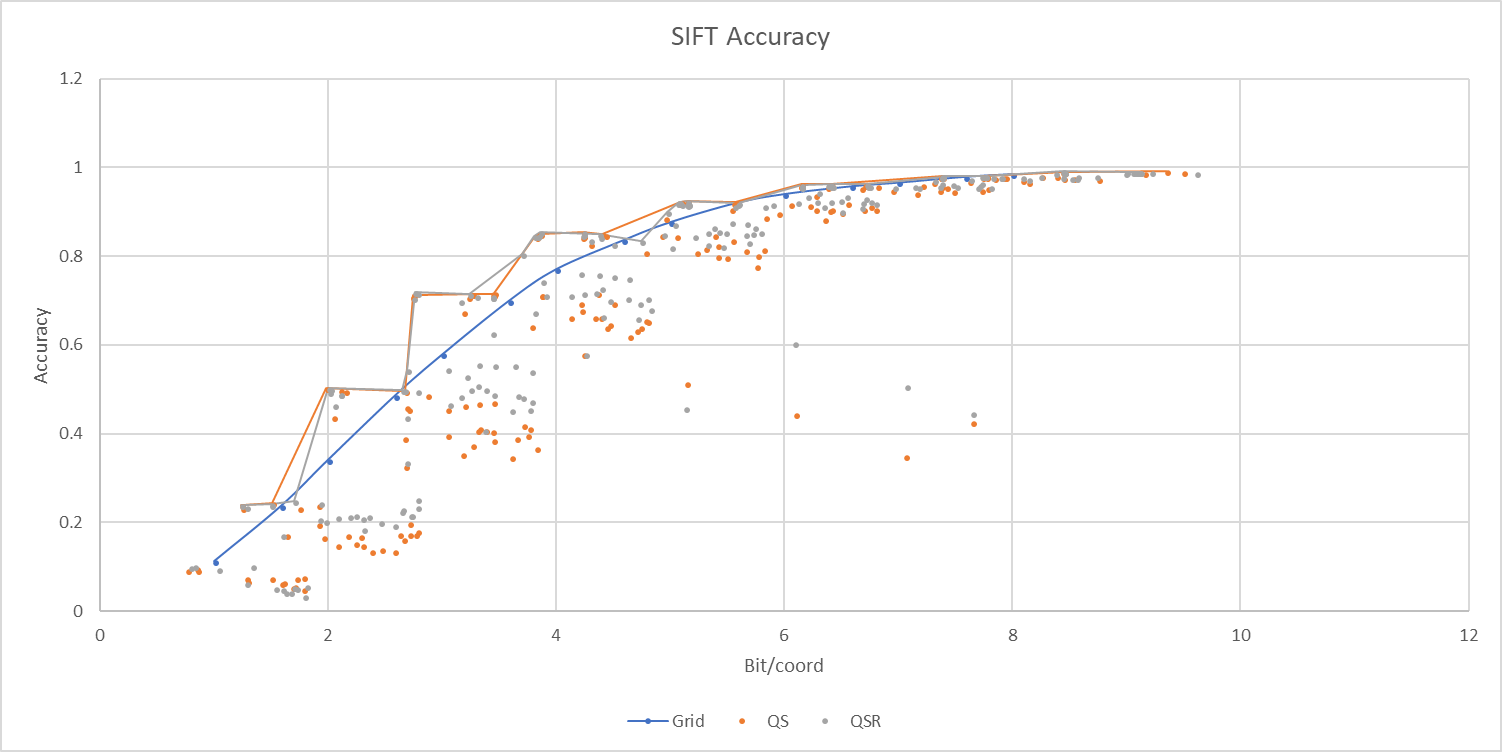
\includegraphics[width=\textwidth]{figures/graphs/sift_accuracy}
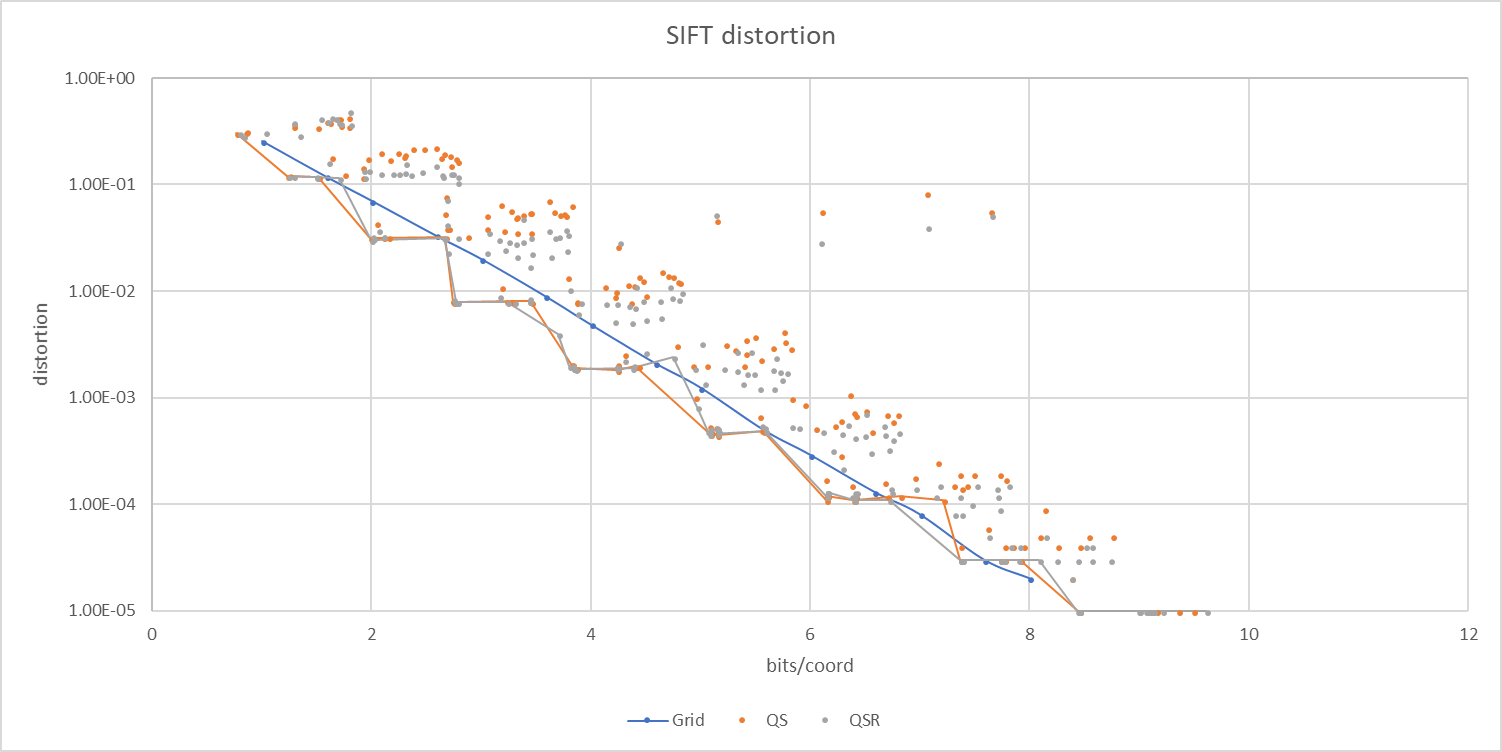
\includegraphics[width=\textwidth]{figures/graphs/sift_distortion}
\caption{Accuracy and distortion from \sift{}}
\label{fig:graph sift}
\end{figure}
The graphs in figure \ref{fig:graph sift} above show that in the best case scenario for \qs{} and \qsr{} are quite similar, while \qsr{} seems to be better in the average case.

\begin{figure}[h!]
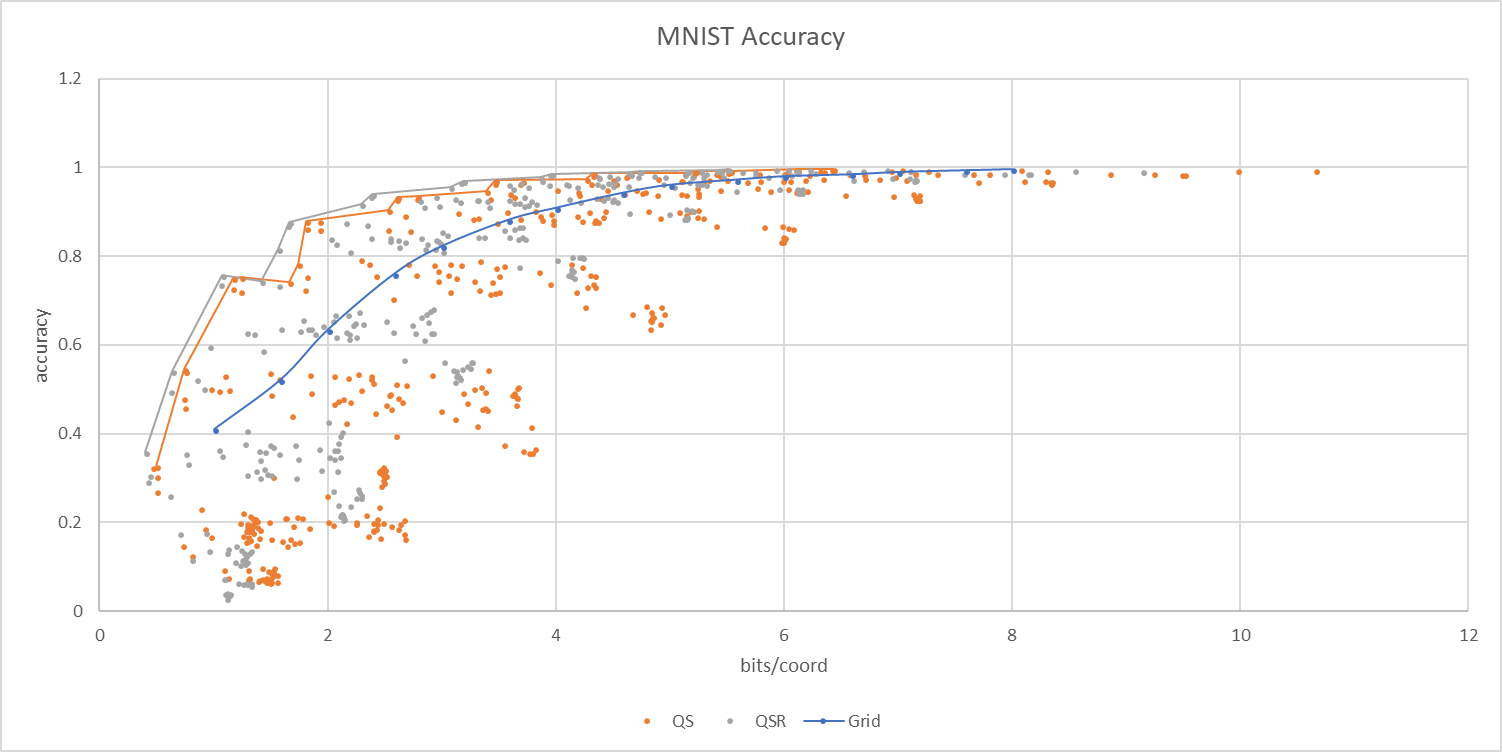
\includegraphics[width=\textwidth]{figures/graphs/mnist_accuracy}
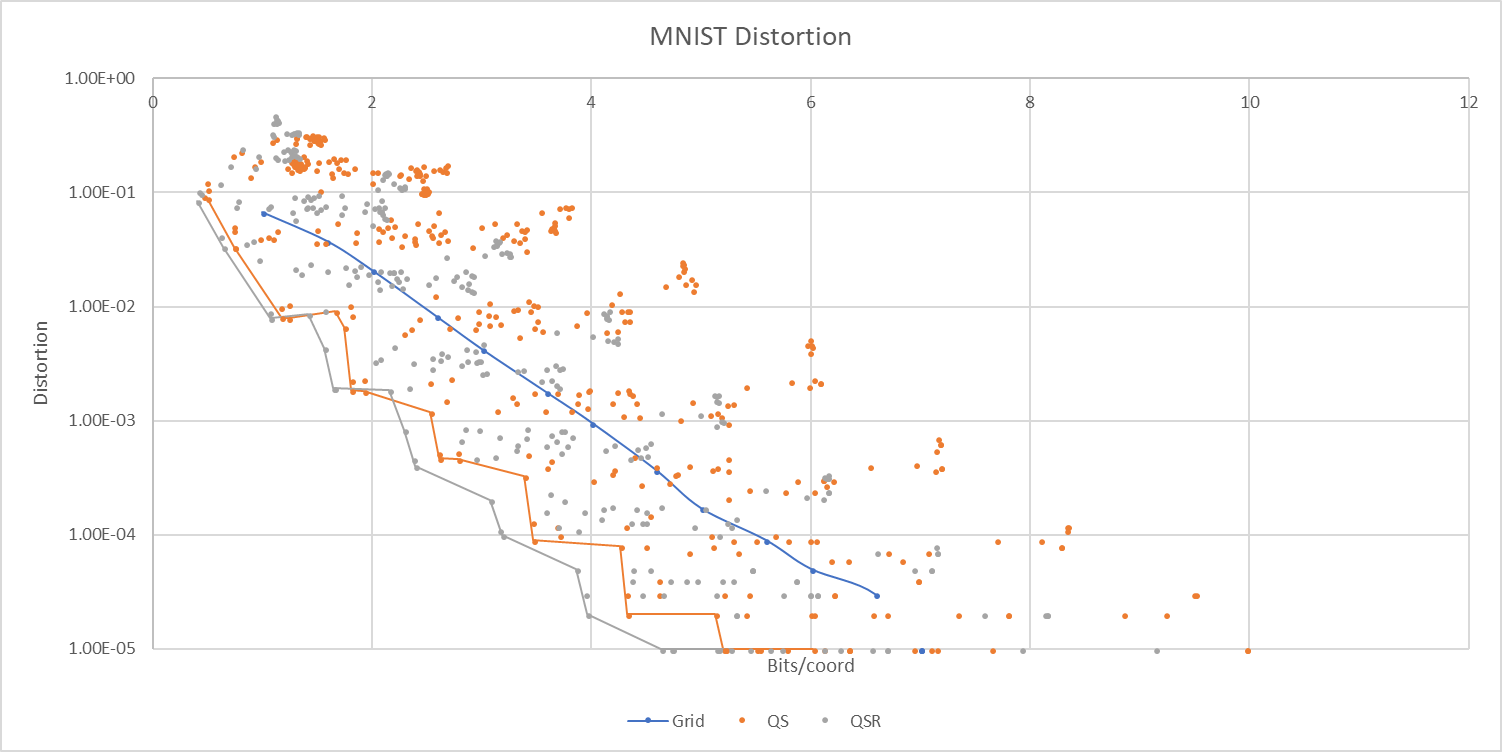
\includegraphics[width=\textwidth]{figures/graphs/mnist_distortion}
\caption{Accuracy and distortion from \mnist{}}
\label{fig:graph mnist}
\end{figure}
\clearpage
Figure \ref{fig:graph mnist} displays that \qsr{} runs are slightly superior to \qs{} in the best case regarding accuracy, and superior in regards to distortion. The average case for \qsr{} in distortion seems superior to the average case in \qs{}, but similar in regards to accuracy.

\begin{figure}[h!]
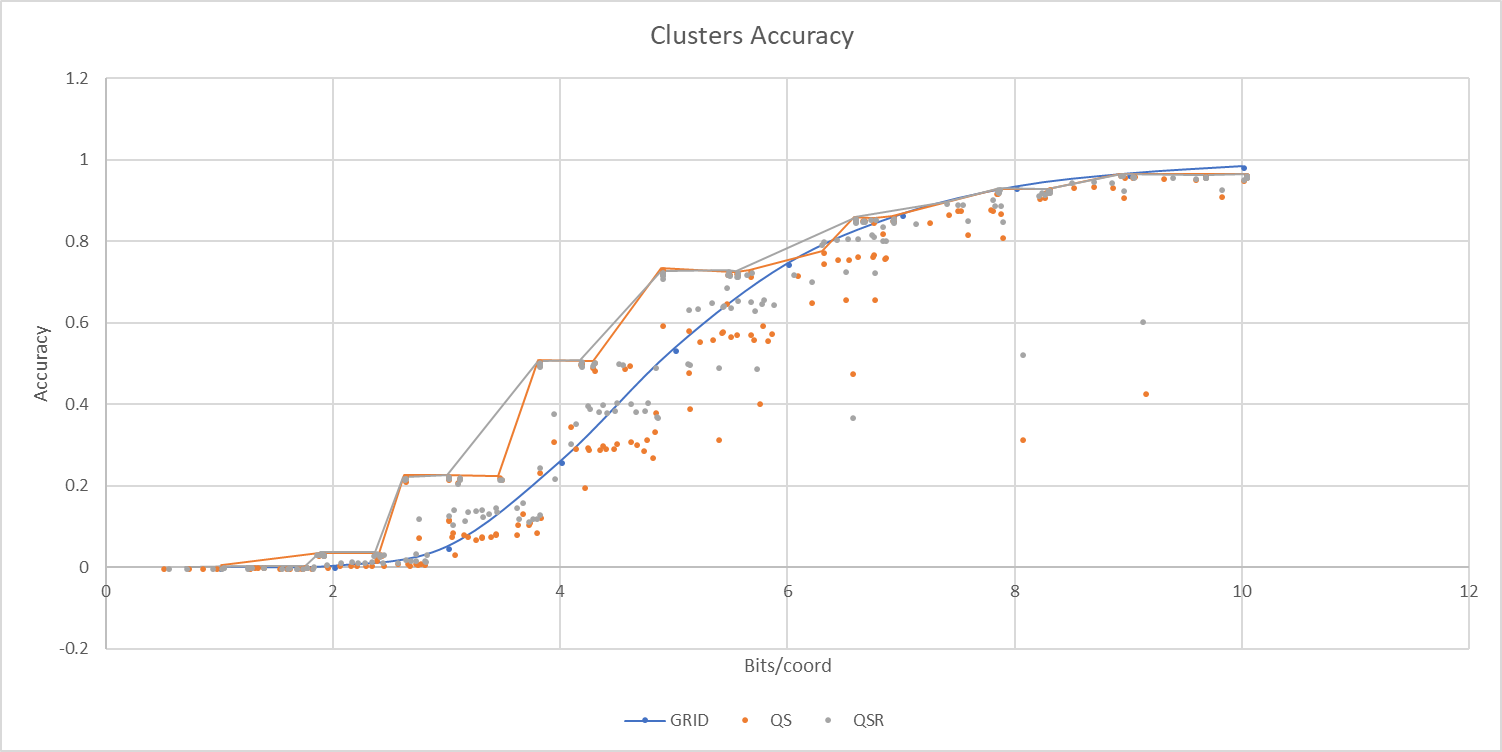
\includegraphics[width=\textwidth]{figures/graphs/clusters_accuracy}
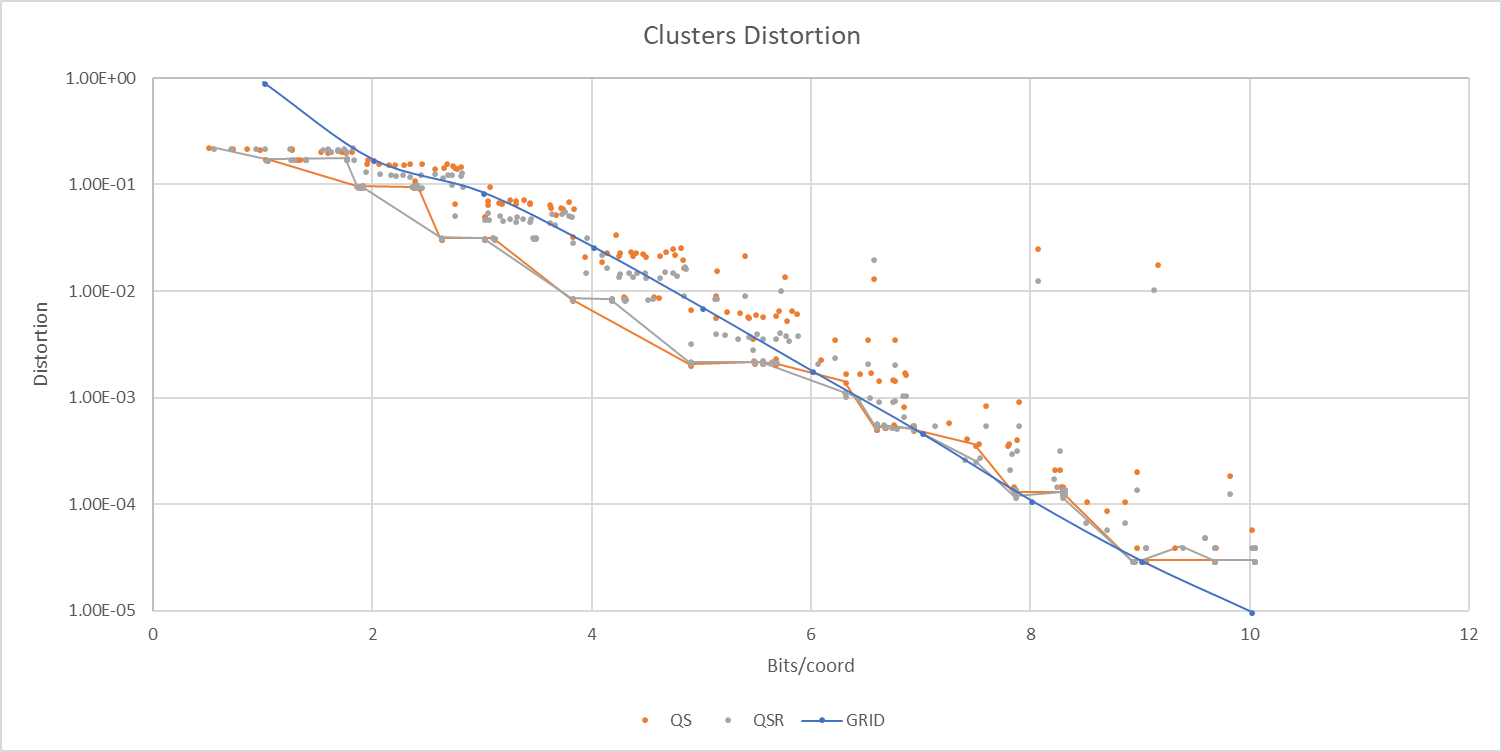
\includegraphics[width=\textwidth]{figures/graphs/clusters_distortion}
\caption{Accuracy and distortion from \clust{}}
\label{fig:graph clust}
\end{figure}
Figure \ref{fig:graph clust} shows that \qs{} and \qsr{} behaves similarly in best case runs for the clusters dataset. However the average case for \qsr{} is slightly superior to the \qs{} average results both regarding accuracy and distortion.
\clearpage
\begin{figure}[h]
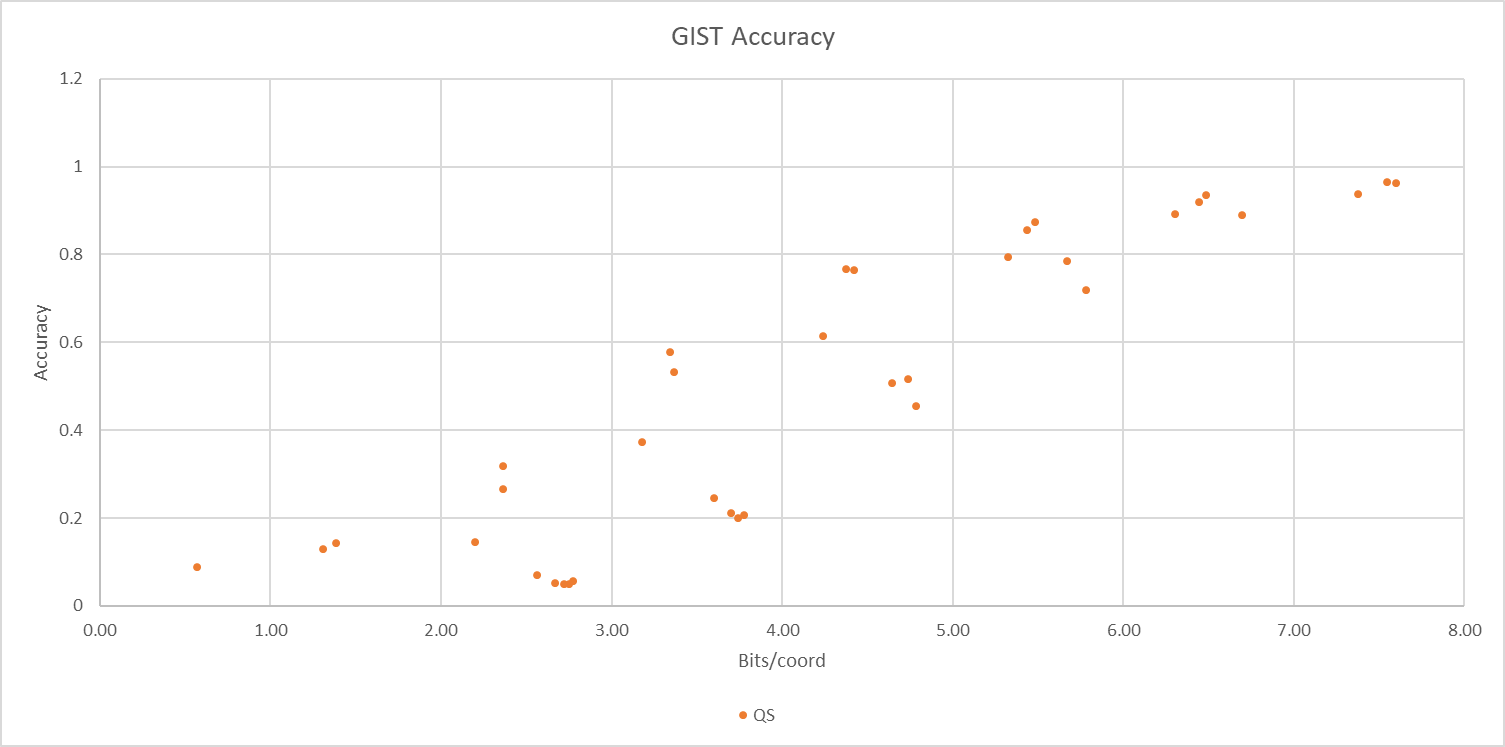
\includegraphics[width=\textwidth]{figures/graphs/gist_accuracy.png}
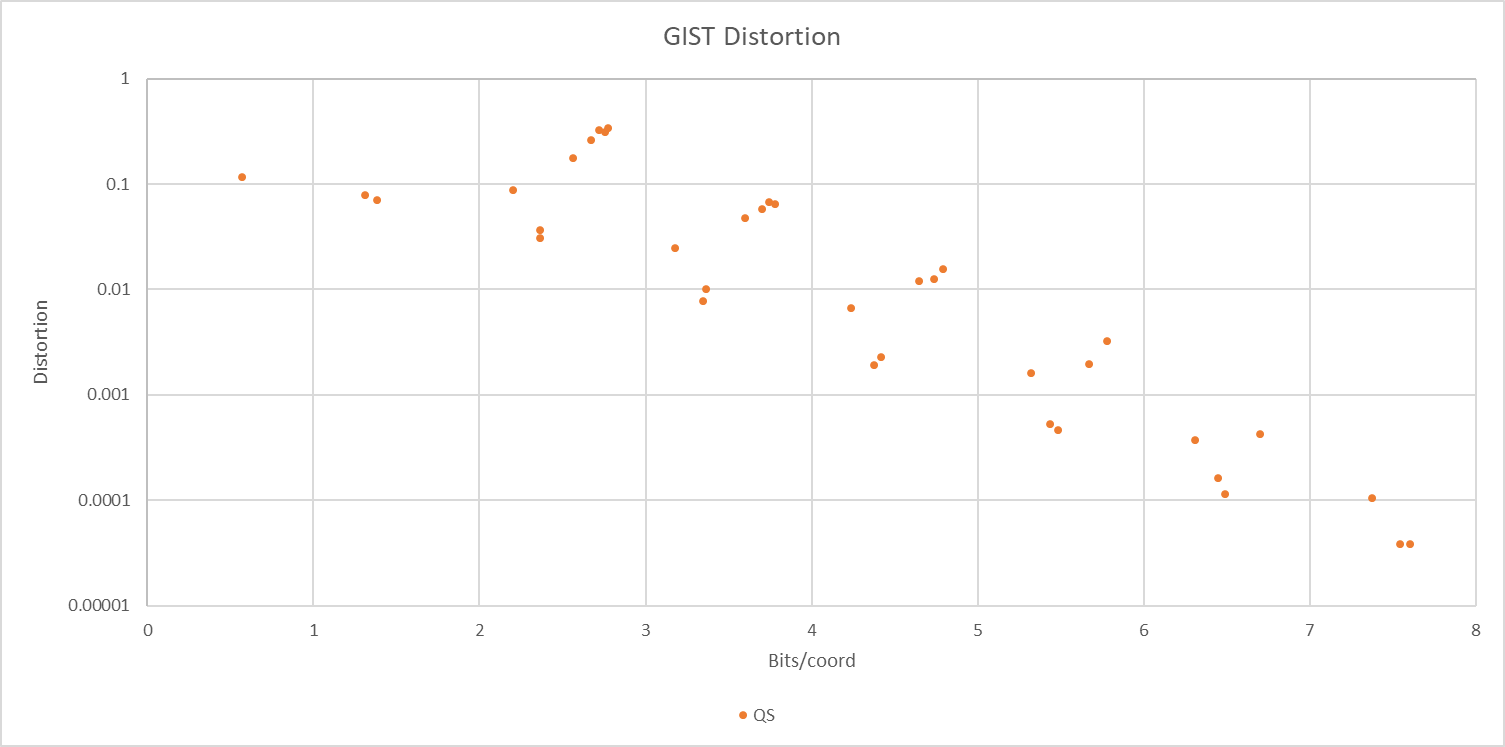
\includegraphics[width=\textwidth]{figures/graphs/gist_distortion.png}
\caption{Accuracy and distortion from \gist{}}
\label{fig:graph gist}
\end{figure}
Figure \ref{fig:graph gist} illustrates that \qs{} behaves similarly to the results in the preceding graphs, in regards to increase in bits per coordinate giving increase in accuracy and decrease in distortion. It is notable however, that a larger number of bits per coordinate is required to gain an accuracy of approximately 1. This is due to the high number of dimensions and the large aspect ratio.
